\section{Setup}
\label{sec:setup}

\begin{figure}[t]
  \centering
  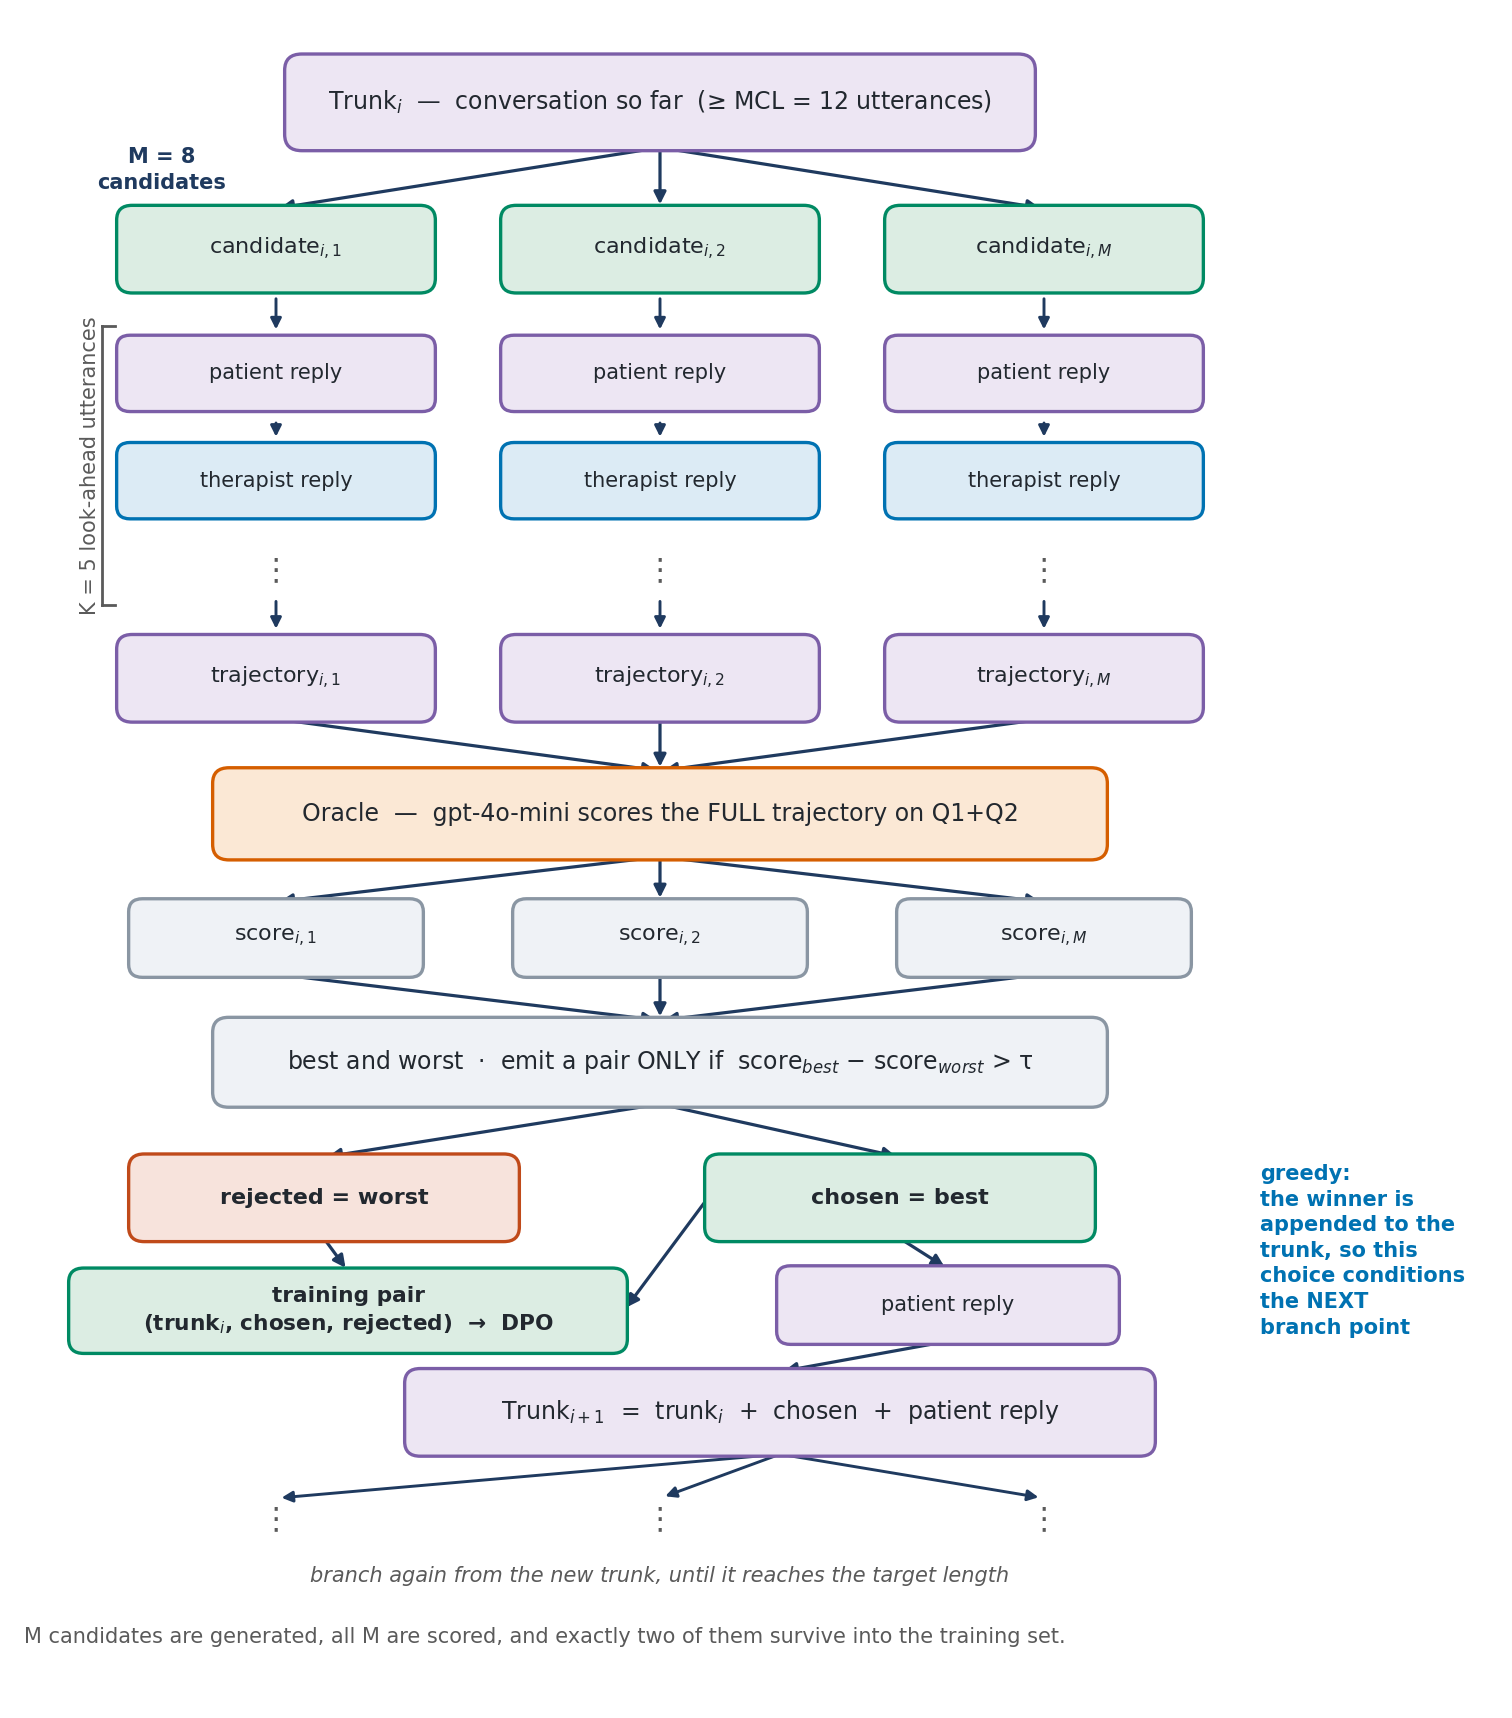
\includegraphics[width=0.42\linewidth]{figures/method_pto_branch.png}\hfill
  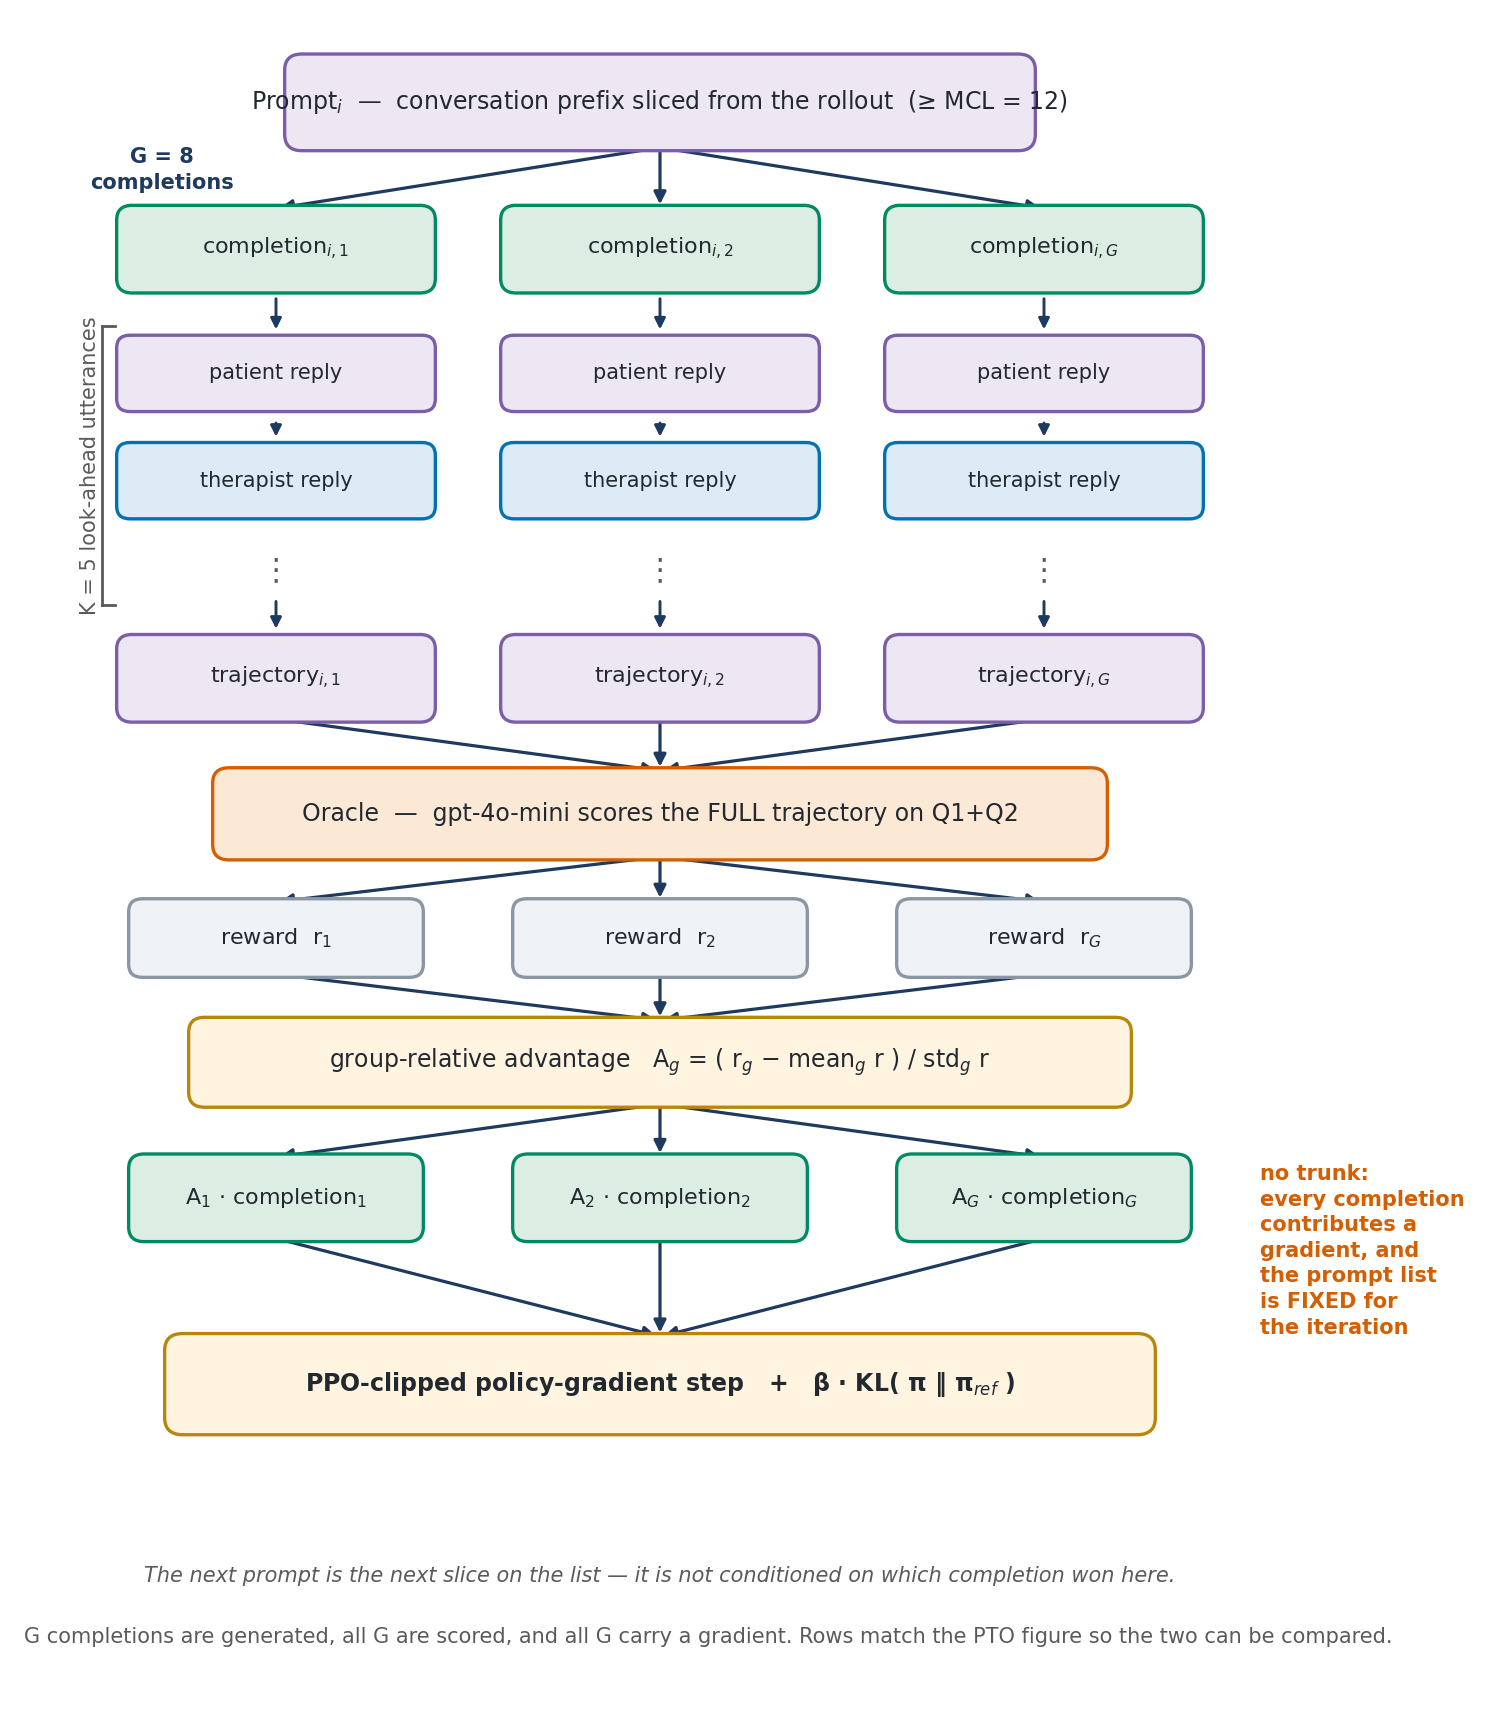
\includegraphics[width=0.42\linewidth]{figures/method_grpo_group.png}
  \caption{PTO (left: $M{=}8$ candidates per turn; best and worst form a DPO pair if their gap
    exceeds $\tau$; the best advances the trunk) and GRPO (right: $G{=}8$ candidates per
    on-policy prefix, all weighted by group-relative advantage) share one step: each candidate is
    rolled $K$ turns forward under the same policy and the oracle grades the result.}
  \label{fig:methods}
\end{figure}

\paragraph{Task and agents.} A Llama-3.2-1B therapist (bf16, LoRA $r{=}16$, learning rate
$10^{-5}$) conducts Motivational Interviewing against a simulated patient. Patient and training
oracle are both \primaryjudge{} (\texttt{gpt-4o-mini-2024-07-18}); the patient is conditioned on
one of 96 persona prompts crossing presenting problem (smoking, obesity), its duration, prior
change attempts, patient gender and age with cooperation level (Cooperative, Warms~up,
Resistant; 32 each), and a conversation runs to a 49-utterance target or until the
patient closes it. The training reward is \QQ{}, the mean of Q1 (session satisfaction) and Q2
(working alliance) from \citet{yosef2024assessing}, filled in by the oracle from the patient's
perspective, as in the poster.

\paragraph{Two optimizers in matched form.} Both are iterative (Figure~\ref{fig:methods}). Each
iteration the current policy generates 96 conversations, one per persona; these are the
evaluation set of that policy and the raw material of its update. \emph{GRPO} slices each
conversation after every patient turn once the transcript holds at least $\mathrm{MCL}{=}12$
utterances (the minimum conversation length, matched across arms), samples $G{=}8$ completions per prompt at temperature $1.2$, scores each, and takes a
clipped policy-gradient step on the group-standardized advantage with a KL penalty
($\beta{=}0.01$) against the iteration-start adapter \citep{shao2024deepseekmath}. \emph{PTO}
seeds a greedy preference tree with the first 12 utterances, samples $M{=}8$ candidates per
therapist turn at the same temperature, scores each, appends the best to the trunk, and emits a
(best, worst) pair when the gap exceeds $\tau{=}0.1$; the pairs train a sigmoid DPO loss
($\beta{=}0.1$) against the same reference \citep{rafailov2023dpo}. Everything else is held
fixed across the four arms (Appendix~\ref{app:repro}).

\paragraph{The manipulation, and one asymmetry.} Under \Kz{} the oracle scores the prefix plus
the candidate turn; under \Kf{} the candidate is first extended by five further simulated turns
--- patient, policy, patient, policy, patient --- generated by the same current policy, and the
oracle scores the extension. This changes what the oracle grades and nothing else, identically
for both optimizers. PTO \Kz{}, PTO \Kf{} and GRPO \Kz{} ran ten iterations; GRPO \Kf{} ran five
and is right-censored (its five iterations cost as much GPU time as GRPO \Kz{}'s ten,
\S\ref{sec:cost}), so every GRPO $K$ contrast here is at iteration $\leq 5$, and a GRPO \Kf{}
endpoint set against a later \Kz{} checkpoint is named as such.

\paragraph{Evaluation.} Every conversation of every model state ($11{+}11{+}11{+}6 = 39$) is
scored on eight instruments: Q1 and Q2 (and their composite), the Working Alliance Inventory
(WAI-SR), the Client Satisfaction Questionnaire (CSQ-8), MI Intervention Satisfaction (MI-SAT)
and the MI Treatment Integrity (MITI) global ratings \citep{moyers2016miti} on Likert scales; PCT,
the patient's percent change talk, i.e.\ change talk as a share of change- plus sustain-talk
utterances (CT/(CT+ST), neutral utterances excluded); and MICI, MI-inconsistent therapist acts
per therapist turn (lower is better). Two graders
score the whole grid ($39 \times 8 \times 96 = 29{,}952$ cells each): the training oracle, and
\heldoutjudge{}, a model from another family that never played the patient and never produced a
training reward; the two are never averaged. Oracle self-repeatability, measured on four \Kz{}
anchor states only (ICC $.990$ Q1, $.976$ Q2, $.916$ MICI), gives the $\pm 0.10$ band drawn in
the figures.

\paragraph{Statistics.} The 96 personas are reshuffled every iteration, so every contrast is
paired on the recovered persona, never on file order: paired mean, Cohen's \dz{}, a
2{,}000-resample bootstrap interval over personas, and a Wilcoxon signed-rank $p$ with Holm
correction across iterations within (grader, method, instrument), the family stated per table
(Appendix~\ref{app:repro}). Tables report $K{=}0$ minus $K{=}5$. Iteration~0 is two
\emph{independent} draws of the untrained model and is the empirical noise floor: on \QQ{} under
the training oracle, $-0.003$ for the PTO pair and $+0.104$ (\dz{} $0.11$, n.s.) for the GRPO
pair.

GPU-hours (cloud A100s) are reconstructed from artifact modification times as generate $+$
build (PTO only) $+$ train per iteration, resume gaps imputed at the phase median; generation is
under-counted by ${\approx}0.1$\,\gpuh{} per iteration and the corrected totals change no
conclusion (Appendix~\ref{app:repro}).
